\documentclass[conference]{IEEEtran}
\usepackage[utf8]{inputenc}
\usepackage[T1]{fontenc}
\usepackage{graphicx}
\usepackage{amsmath,amssymb}
\usepackage{booktabs}
\usepackage{xcolor}
\usepackage{url}
\usepackage[hidelinks]{hyperref}
\usepackage{tabularx}
\usepackage{array}

% ---------------------------------------------------------------------------
% \BEREN{...}: a part only Beren may write (Section 11 of the brief: AI may not
% write the corner-selection logic or the Stage 4 comparison analysis).
% Delete the box when the text is in place.
% ---------------------------------------------------------------------------
\newcommand{\BEREN}[1]{\par\noindent\fcolorbox{red}{red!6}{\parbox{\dimexpr\linewidth-2\fboxsep-2\fboxrule}{\footnotesize\textbf{\textcolor{red}{[TO BE WRITTEN BY THE STUDENT]}} #1}}\par}

\newcommand{\TBD}{\textcolor{red}{[fill in]}}
\graphicspath{{figs/}}
\raggedbottom

\begin{document}

\title{SudokuScan: From a Photograph of a Printed Puzzle\\to a Digital $9\times9$ Grid}

\author{\IEEEauthorblockN{Zeyneb Beren Kece}
\IEEEauthorblockA{Computer Engineering, MEF University, Istanbul\\
Student no.\ 042401168 --- COMP 482 Computer Vision, Fall 2026, Project 1}}

\maketitle

\begin{abstract}
SudokuScan reads a printed sudoku from a single phone photograph. It finds the four outer corners of the puzzle with the Harris detector, rectifies the grid with an exact three-point affine map (A3), a least-squares four-point affine map (A4) and a homography (H4), splits the H4 image into 81 cells, decides empty versus filled before OCR, reads the digits with Tesseract and checks the result against the sudoku rules. On the 20-image development set the mean corner error is 0.063\,\% of the puzzle side, cell accuracy is 99.94\,\% and 19 of 20 grids are exact; on 12 personal photographs the corner error is 0.111\,\% and all 12 grids are exact. Across 31 annotated photos tilted up to $55^\circ$, homography rectification kept cell accuracy at 99.9--100\,\%, while both affine models fell to about 60\,\% beyond $30^\circ$, so affine rectification suffices only for near-frontal views.
\end{abstract}

% ===========================================================================
\section{Introduction}
% ===========================================================================
A photographed sudoku is a plane seen through a perspective camera. The printed grid gives strong, known structure, but the photograph adds what makes the problem hard: the puzzle can sit anywhere in the frame, be rotated in the image plane, be seen obliquely so that the square becomes a general quadrilateral, lie under a shadow, and share the frame with newspaper text, crosswords and other rectangles. The output must be produced automatically, with no per-image parameters, in at most 20\,s on a CPU.

The pipeline has six stages, each a separate module in \texttt{pipeline/}:
(1)~preprocessing to a 1200\,px working image with illumination normalisation;
(2)~Harris response, candidate points and automatic selection of the four outer corners, refined with \texttt{cornerSubPix};
(3)~A3, A4 and H4 rectification to $450\times450$\,px;
(4)~a measured comparison of the three models;
(5)~cell extraction, an explicit empty-cell criterion and Tesseract OCR on prepared cells;
(6)~a row, column and box validity check.
Two safeguards were added after the first full runs: a grid check that rejects quadrilaterals which are not a $9\times9$ grid with at least 17 givens, and an orientation step that chooses among the four cyclic corner orders by OCR confidence.



Section~\ref{sec:results} summarises the results: the corner error stays far below the 1.5\,\% band on both sets, the empty-cell F1 is 0.9995 and 1.0000, and no image crashes. The main limitations are page curl, strong blur and the runtime on a single CPU core (Section~\ref{sec:failures}).

% ===========================================================================
\section{Corner Detection}
\label{sec:corners}
% ===========================================================================
\subsection{Preprocessing}
Every input is downscaled so that its long side is 1200\,px (the scale factor $s$ is kept), converted to grey and smoothed with a Gaussian whose kernel is 0.5\,\% of the long side. Uneven illumination is removed by dividing the image by a strongly blurred copy of itself (kernel 12\,\% of the long side, larger than one cell, so that the estimate follows the light and not the ink). All kernel sizes are fractions of the image size, so the same code runs on a 1600\,px development image and a 5712\,px phone photograph. Corners found in the working image are mapped back with $p_\text{orig} = (p_\text{work}+0.5)/s - 0.5$, which respects pixel centres.

\subsection{Harris response and candidates}
\texttt{cv2.cornerHarris} computes, for each pixel, $R=\det M - k\,(\operatorname{tr} M)^2$, where $M$ is the structure tensor of the Sobel gradients summed over a \texttt{blockSize} window. $R$ is large and positive at corners, negative along edges and near zero in flat regions. The chosen values are \texttt{blockSize} $=0.004\times$ long side (5\,px at 1200\,px), \texttt{ksize} $=3$ and $k=0.04$. Candidates are the pixels with $R > 0.01\,R_{\max}$ that are equal to their dilation over a window of 1\,\% of the long side (non-maximum suppression); touching maxima are merged with connected components. A photograph yields 108--432 candidates on the development set (Fig.~\ref{fig:harris}, Appendix~\ref{app:tables}); they come from grid intersections, digit strokes, background text and the page edge. The response map, all candidates and the four selected corners are saved as \texttt{<name>\_harris.png}.



\subsection{Automatic selection of the four outer corners}
A contour search decides where each corner is. Harris and \texttt{cornerSubPix} decide its exact position, so the final corners always come from \texttt{cv2.cornerHarris}.

After resizing to a 1200\,px long side, blurring and removing shading, an adaptive threshold exposes the grid lines. Only convex four-vertex contours are kept. The puzzle is taken to be the smallest quadrilateral that covers at least 2\,\% of the image and contains at least three smaller quadrilaterals. The paper and any printed frame contain the same cells but are larger, while notes boxes contain none.

Each corner of this quadrilateral is snapped to the nearest strong local maximum of the Harris response (\texttt{blockSize} 5\,px, $k=0.04$) within $\pm6$\,px. On a thick border the strongest peak is often the inner corner. The point is then refined with \texttt{cornerSubPix} on the full-resolution image, which reduces the mean corner error from 0.51\,\% to 0.06\,\%.

A candidate is rejected (\texttt{not\_found}) unless its rectification shows a $9\times9$ grid and at least 17 filled cells. The corner order is set by the orientation that gives the most confident digit readings.

Mean corner error: 0.063\,\% on the 20 development images and 0.111\,\% on the 12 personal photos.


\subsection{Parameter study}


\begin{table}[t]
\centering\footnotesize
\caption{\texttt{blockSize} on all 32 annotated images: final corner error.}
\label{tab:block}
\begin{tabular}{@{}r r r r@{}}
\toprule
Ratio & Mean (\%) & Worst (\%) & Images $>0.4$\,\%\\
\midrule
0.003 & 0.093 & 0.557 & 1\\
\textbf{0.004} & 0.081 & 0.183 & 0\\
0.005 & 0.345 & 0.955 & 11\\
0.007 & 0.841 & 1.526 & 30\\
0.012 & 1.594 & 2.475 & 32\\
\bottomrule
\end{tabular}
\end{table}

\begin{figure*}[t]
\centering
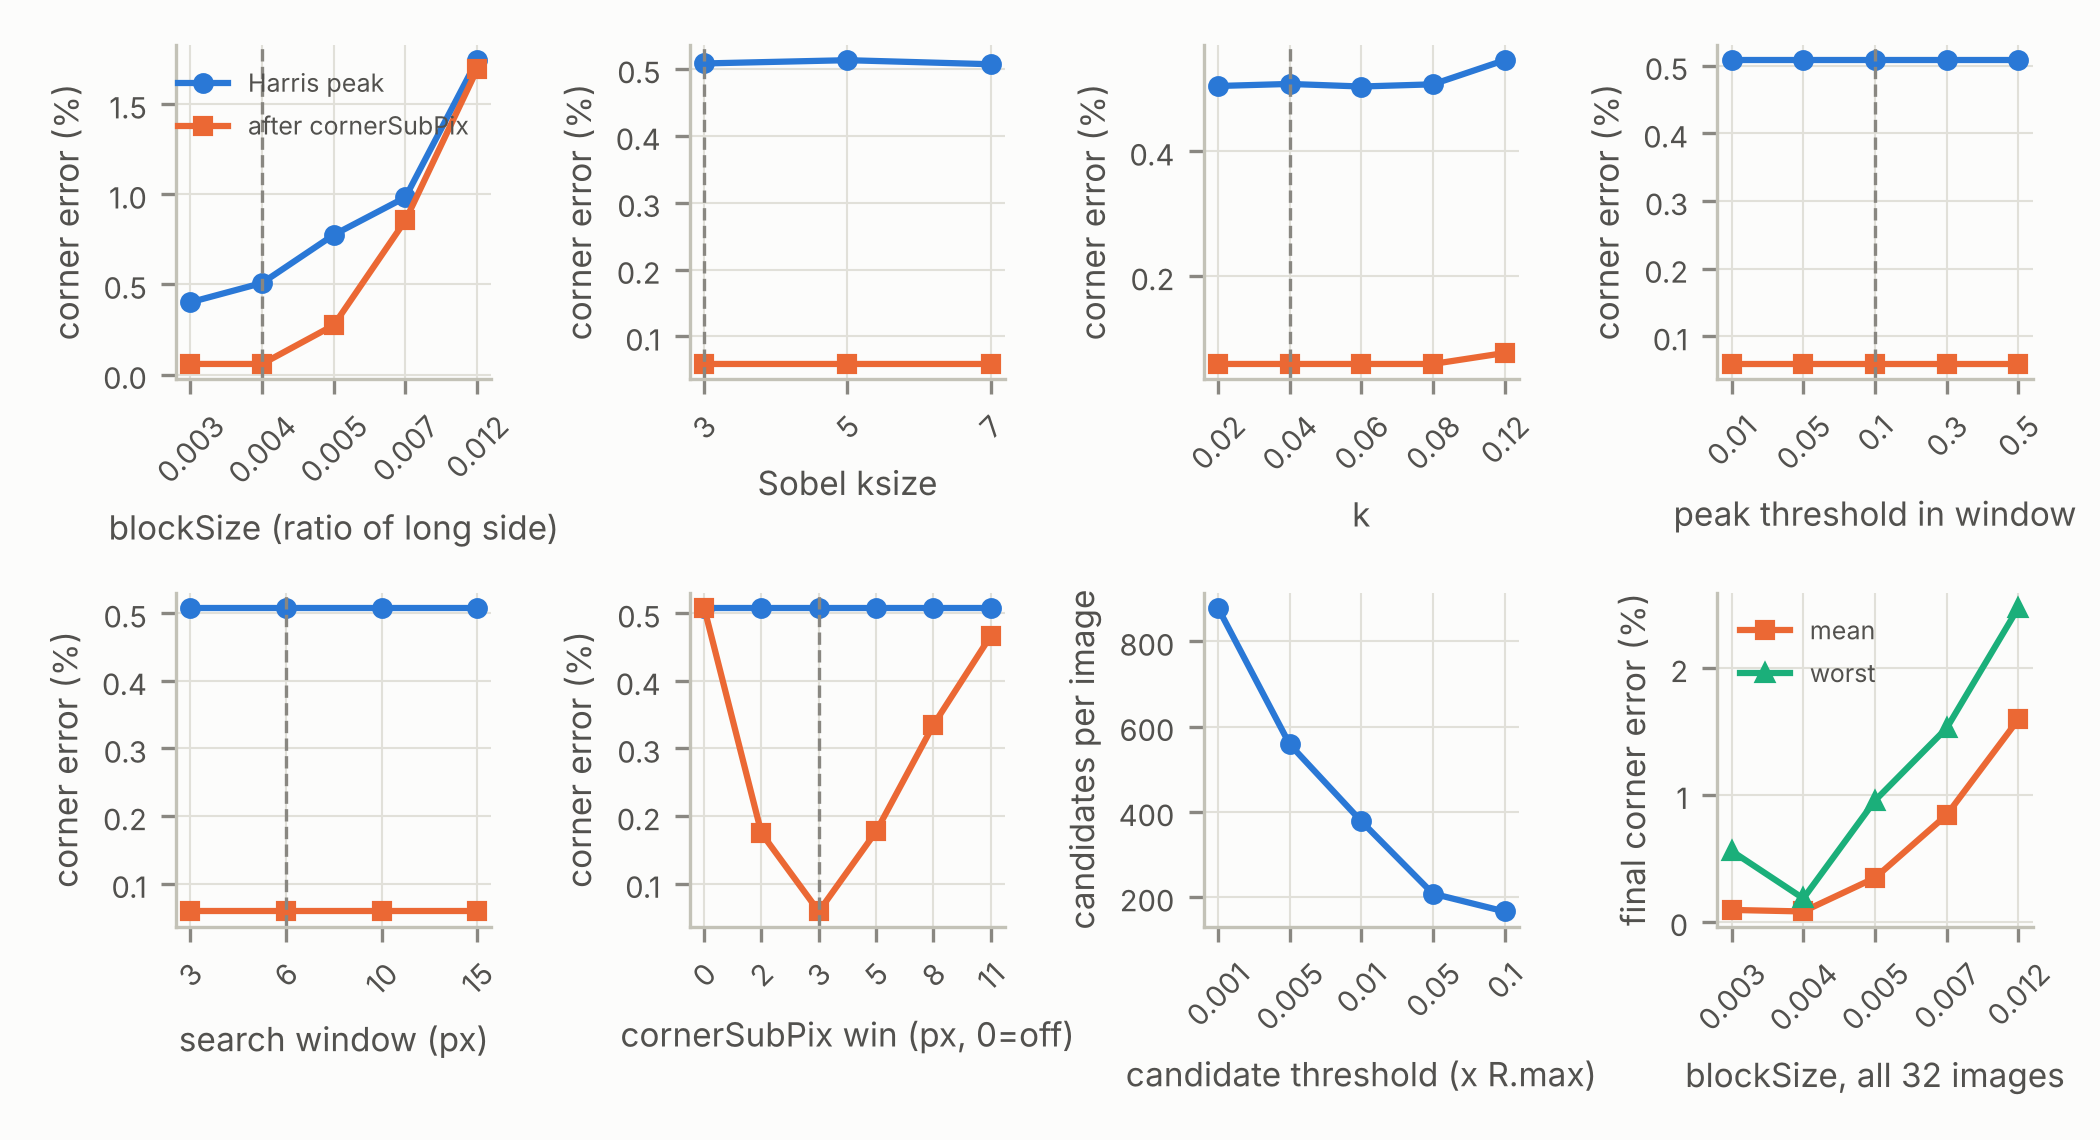
\includegraphics[width=0.78\textwidth]{harris_params.png}
\caption{Harris parameter study. Blue: error of the snapped Harris peak; orange: final error after \texttt{cornerSubPix}; dashed line: chosen value. Bottom right: \texttt{blockSize} on all 32 annotated images.}
\label{fig:harris-params}
\end{figure*}

Each parameter was varied on its own while the others were held at their chosen values. Eight images were used: frontal, oblique, rotated, unevenly lit, cluttered and curled. Errors are measured before and after \texttt{cornerSubPix} (Fig.~\ref{fig:harris-params}; all values in Table~\ref{tab:harris}, Appendix~\ref{app:tables}).
\begin{itemize}
\item \texttt{blockSize} $=5$\,px (0.4\,\% of the long side). Larger windows pull the peak into the thick border: at 15\,px the error is 1.7\,\% even after refinement. On the eight images 3\,px was equally good, but on all 32 annotated images it chose a wrong peak once (0.56\,\%). 5\,px had a worst case of 0.18\,\% (Table~\ref{tab:block}).
\item \texttt{ksize} $=3$, $k=0.04$. Neither changes the result between 3--7 and 0.02--0.08 (0.059\,\%). We keep the standard values; $k=0.12$ starts to degrade the result (0.076\,\%).
\item Thresholds. The candidate threshold only changes how many points are drawn in the debug image (879 to 166) and the peak threshold has no effect, because the corner is searched locally. The search radius (3--15\,px) is also irrelevant, since on these images the selected peak always lies within 3\,px.
\item \texttt{cornerSubPix} window $=3$\,px is the most sensitive choice. It lowers the error from 0.51\,\% without refinement to 0.059\,\%. Smaller windows (2\,px) do not reach the corner, and larger ones (5--11\,px) include the inner edge of the border (0.18--0.47\,\%).
\end{itemize}


\subsection{Failure cases of the corner stage}
\begin{enumerate}
\item \emph{Harris peak shifted inward.} On a thick border the Harris maximum lies inside the line, not on its outer corner. Without refinement the mean error is 0.51\,\%, roughly constant over all four corners. This is a systematic bias, not a wrong candidate. \texttt{cornerSubPix} on the full-resolution image removes it (0.06\,\%).
\item \emph{Rotation beyond $45^\circ$} (\texttt{s042401168\_09}, \texttt{\_11}). The quadrilateral was found correctly, but $x+y$ picked the image's top-left instead of the puzzle's, so all four corners were one position off (100\,\% error, sideways grid; Fig.~\ref{fig:corner-failures}a, Appendix~\ref{app:tables}). Fix: the corner order is chosen by OCR confidence over the four orientations (0.18\,\% and 0.15\,\%; Fig.~\ref{fig:corner-failures}b). In the stress test, all 32 images rotated by $90^\circ$, $180^\circ$ and $270^\circ$ were found.
\item \emph{Grids that are not sudokus.} A $6\times4$ table and a tic-tac-toe board passed the ``smallest quadrilateral with inner quadrilaterals'' rule, and the board was reported as \texttt{valid}. Fix: a $9\times9$ line check on the rectified image (13--20 of 20 lines on real puzzles, 6 and 8 on the fakes).
\item \emph{Blur, darkness and low resolution.} When the thin cell lines are blurred or faint, the cells no longer close into quadrilaterals. The puzzle then contains fewer than three inner shapes and is rejected (Fig.~\ref{fig:corner-failures}c). This happened in 5 of 32 blurred images, 1 darkened, 1 noisy and 1 at 25\,\% size; two of these have a different cause (blurred \texttt{s042401168\_07} is rejected by the $9\times9$ line check, and in darkened \texttt{s042401168\_12} the outer border itself does not close). These are safe failures (\texttt{not\_found}). A more dangerous case is blurred \texttt{dev\_13}: its corners were correct, but the orientation step picked $180^\circ$ (141\,\% error). Possible fix: close gaps morphologically before contour search, and require a larger confidence margin (currently 10 points) before accepting a non-zero rotation.
\item \emph{Parameter sensitivity.} With a 3\,px Harris window, \texttt{s042401168\_07} snapped to a wrong peak (0.56\,\%), although eight test images had suggested 3\,px was best. This is why the final 5\,px value was checked on all 32 images.
\end{enumerate}




% ===========================================================================
\section{Rectification}
\label{sec:rect}
% ===========================================================================
The four corners are mapped to a $450\times450$ target (50\,px per cell). Following the pixel-centre convention of the annotations, the target corners are $(-0.5,-0.5)$, $(449.5,-0.5)$, $(449.5,449.5)$ and $(-0.5,449.5)$, so each cell covers exactly $50\times50$ pixels.

\textbf{Affine map.} In homogeneous coordinates an affine map is a $3\times3$ matrix with last row $[0\;0\;1]$ and six free entries $a_{11},a_{12},a_{21},a_{22},t_x,t_y$. It has six unknowns. Each point correspondence gives two linear equations, so three non-collinear pairs determine it exactly. Because the last row is $[0\;0\;1]$, $w$ stays 1: lines stay lines, parallel lines stay parallel and ratios along a line are kept. An affine map can turn a square into any parallelogram, but never into a general quadrilateral, and it cannot create a vanishing point.

\textbf{Homography.} A homography is a full $3\times3$ matrix $H$ with $\mathbf{x}'\sim H\mathbf{x}$. Since $H$ and $\lambda H$ describe the same mapping, it has $9-1=8$ degrees of freedom, so four pairs (no three collinear) are needed. The third row makes the denominator $h_{31}x+h_{32}y+h_{33}$ depend on the point: parallel lines may converge to a vanishing point and a square may map to any convex quadrilateral. The perspective image of a plane is exactly a homography, so H4 is the correct model for a flat page; an affine map is only an approximation of it.

\textbf{The three models.}
A3 uses \texttt{cv2.getAffineTransform} on TL, TR and BL; the unused BR corner is pushed through the same matrix and its distance from $(449.5,449.5)$ is reported. An affine map forces $\text{BR}=\text{TR}+\text{BL}-\text{TL}$, so the whole deviation of the photographed quadrilateral from a parallelogram shows up at BR.
A4 uses \texttt{cv2.estimateAffine2D} on all four corners: 8 equations, 6 unknowns, solved in the least-squares sense; the RMS residual $\sqrt{\tfrac14\sum_i\lVert A\mathbf{p}_i-\mathbf{q}_i\rVert^2}$ is reported. H4 uses \texttt{cv2.getPerspectiveTransform} and maps the four corners onto the target exactly (Section~\ref{sec:compare}-B). A3 and A4 are warped with \texttt{cv2.warpAffine}, H4 with \texttt{cv2.warpPerspective}.

\textbf{Residuals.} With the detected corners, the A3 fourth-corner error ranges from 15.7 to 259.1\,px on the development set and from 2.1 to 388.8\,px on the personal set; the A4 RMS residual ranges from 4.0 to 54.6\,px and from 0.5 to 62.8\,px. Both are written to every \texttt{\_result.json}. Section~\ref{sec:compare} relates them to the viewing angle.

% ===========================================================================
\section{Affine Versus Homography}
\label{sec:compare}
% ===========================================================================
\subsection{Obliqueness measure}
Obliqueness is the angle between the puzzle plane and the image plane, recovered from the homography. The homography $H$ maps the unit square to the four corners. With the principal point at the image centre, $H = K\,[\mathbf{r}_1\;\mathbf{r}_2\;\mathbf{t}]$ with $K=\operatorname{diag}(f,f,1)$. The conditions $\lVert\mathbf{r}_1\rVert=\lVert\mathbf{r}_2\rVert$ and $\mathbf{r}_1\perp\mathbf{r}_2$ give the focal length $f$. The plane normal is $\mathbf{n}=K^{-1}\mathbf{h}_1\times K^{-1}\mathbf{h}_2$, and the tilt is the angle between $\mathbf{n}$ and the optical axis.

For the personal photos, $f$ is taken from the EXIF 35\,mm-equivalent focal length ($f_\text{px}=f_{35}\cdot\text{long side}/36$), because estimating $f$ from $H$ is unstable near frontal views. On the oblique views the estimate agrees with EXIF (2694\,px vs.\ 2688\,px).

On the development set, which provides true tilt and pan, the measure has a median error of $0.02^\circ$ against $\arccos(\cos\text{tilt}\cdot\cos\text{pan})$. The one exception is \texttt{dev\_14}, where the focal estimate fails ($35.4^\circ$ instead of $18.0^\circ$); it is excluded from the tilt plots. Among four candidate measures it ranked highest against the true angle (Spearman 0.991; side ratio 0.961, mean corner-angle deviation 0.980, parallelogram deviation 0.968).


\subsection{How the measures are computed}
All three models are fitted to the annotated corners, so corner-detection error does not enter the comparison. The target is $450\times450$\,px with corners at $(-0.5,-0.5)\ldots(449.5,449.5)$.
\begin{itemize}
\item \emph{A3 fourth-corner error:} the exact affine from TL, TR and BL maps BR, and the result is the Euclidean distance to the target BR in pixels.
\item \emph{A4 RMS residual:} \texttt{estimateAffine2D} with a very large RANSAC threshold, so all four points are inliers. This was verified against \texttt{np.linalg.lstsq} (maximum difference $4\cdot10^{-12}$). The residual is $\text{RMS}=\sqrt{\tfrac14\sum_i\lVert A\mathbf{p}_i-\mathbf{q}_i\rVert^2}$.
\item \emph{H4:} \texttt{getPerspectiveTransform}. It reproduces the four corners to within $3\cdot10^{-5}$\,px.
\item \emph{Grid regularity:} on the rectified image the grey ``darkness'' (inverted, shading-corrected) is opened with horizontal and vertical kernels 0.4 of a cell long, which removes the digits. Ten peaks are taken from each projection profile. Spacing error is $|\text{gap}-50\,\text{px}|$, and straightness is the spread of each line's position across three strips. Areas outside the photo are masked.
\item \emph{OCR accuracy:} the same OCR on a $900\times900$ warp from each model, scored as the fraction of the 81 cells that are correct.
\end{itemize}








\begin{figure*}[t]
\centering
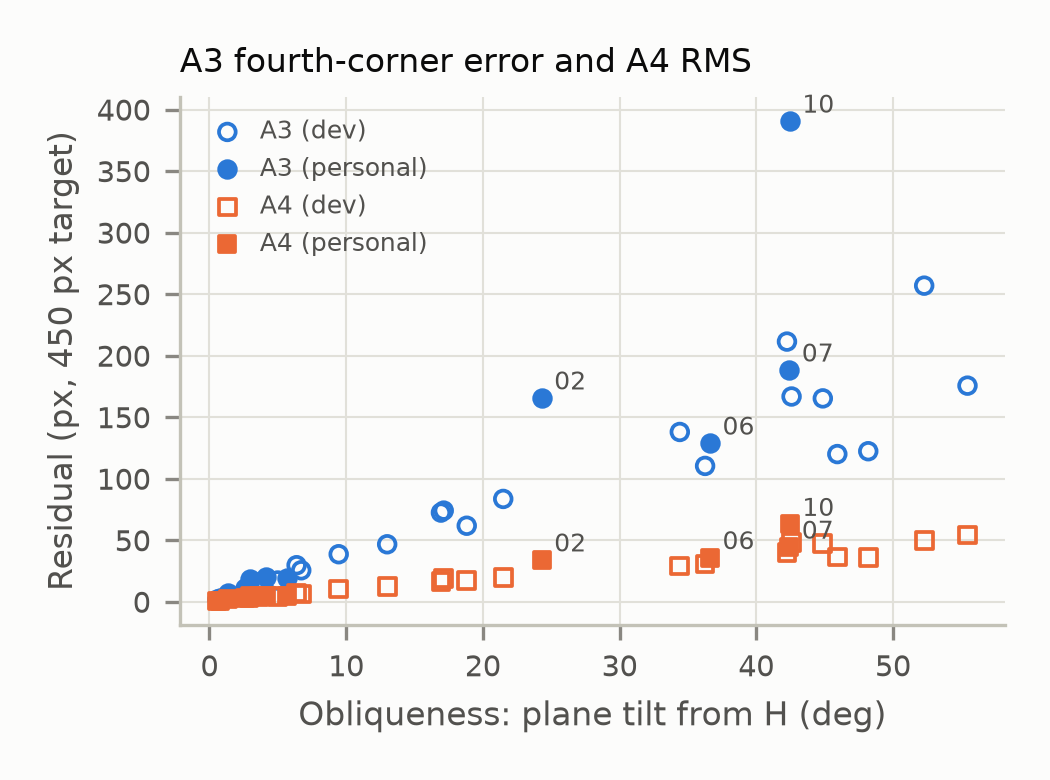
\includegraphics[width=0.325\textwidth]{residual_vs_tilt.png}\hfill
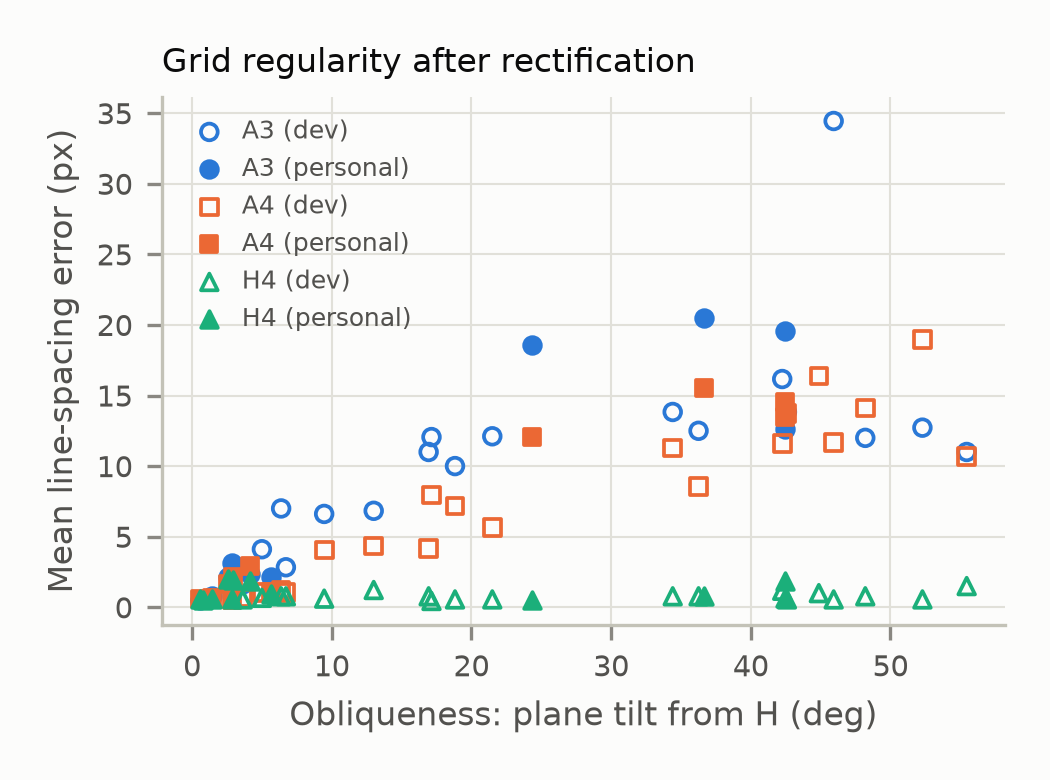
\includegraphics[width=0.325\textwidth]{grid_vs_tilt.png}\hfill
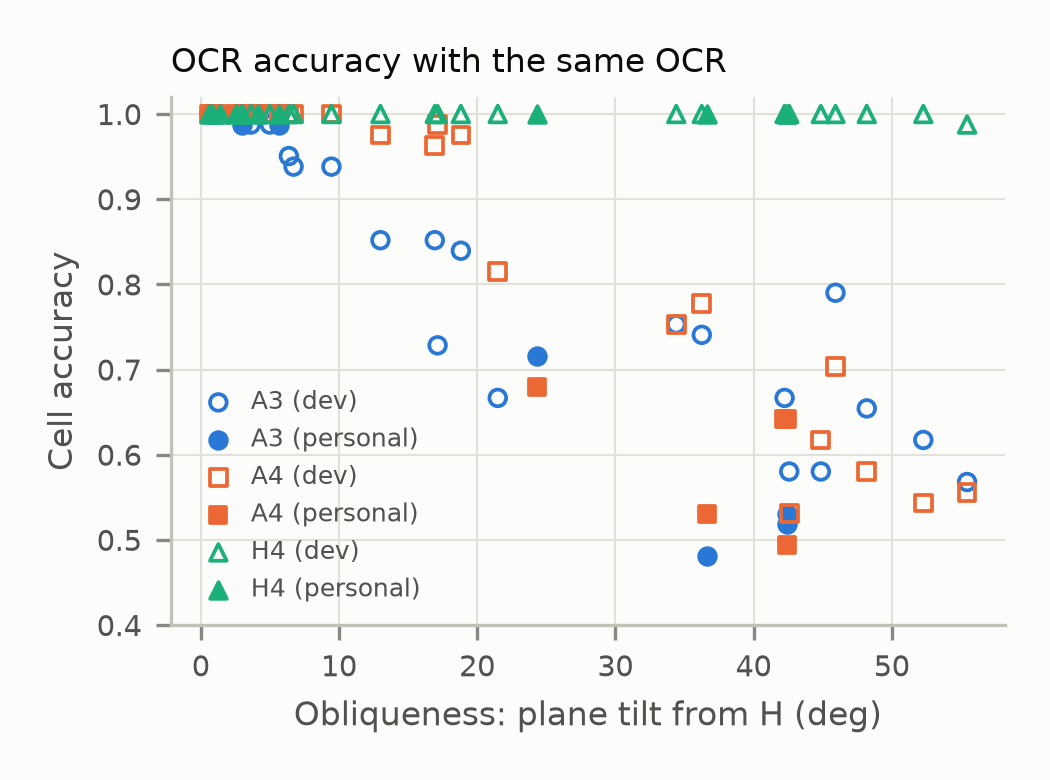
\includegraphics[width=0.325\textwidth]{ocr_vs_tilt.png}
\caption{Stage 4 measures against obliqueness on 32 images (annotated corners). Left: A3 fourth-corner error and A4 RMS residual. Middle: grid-line spacing and straightness after rectification. Right: OCR cell accuracy on the A3, A4 and H4 rectifications.}
\label{fig:measures}
\end{figure*}
\begin{figure*}[t]
\centering
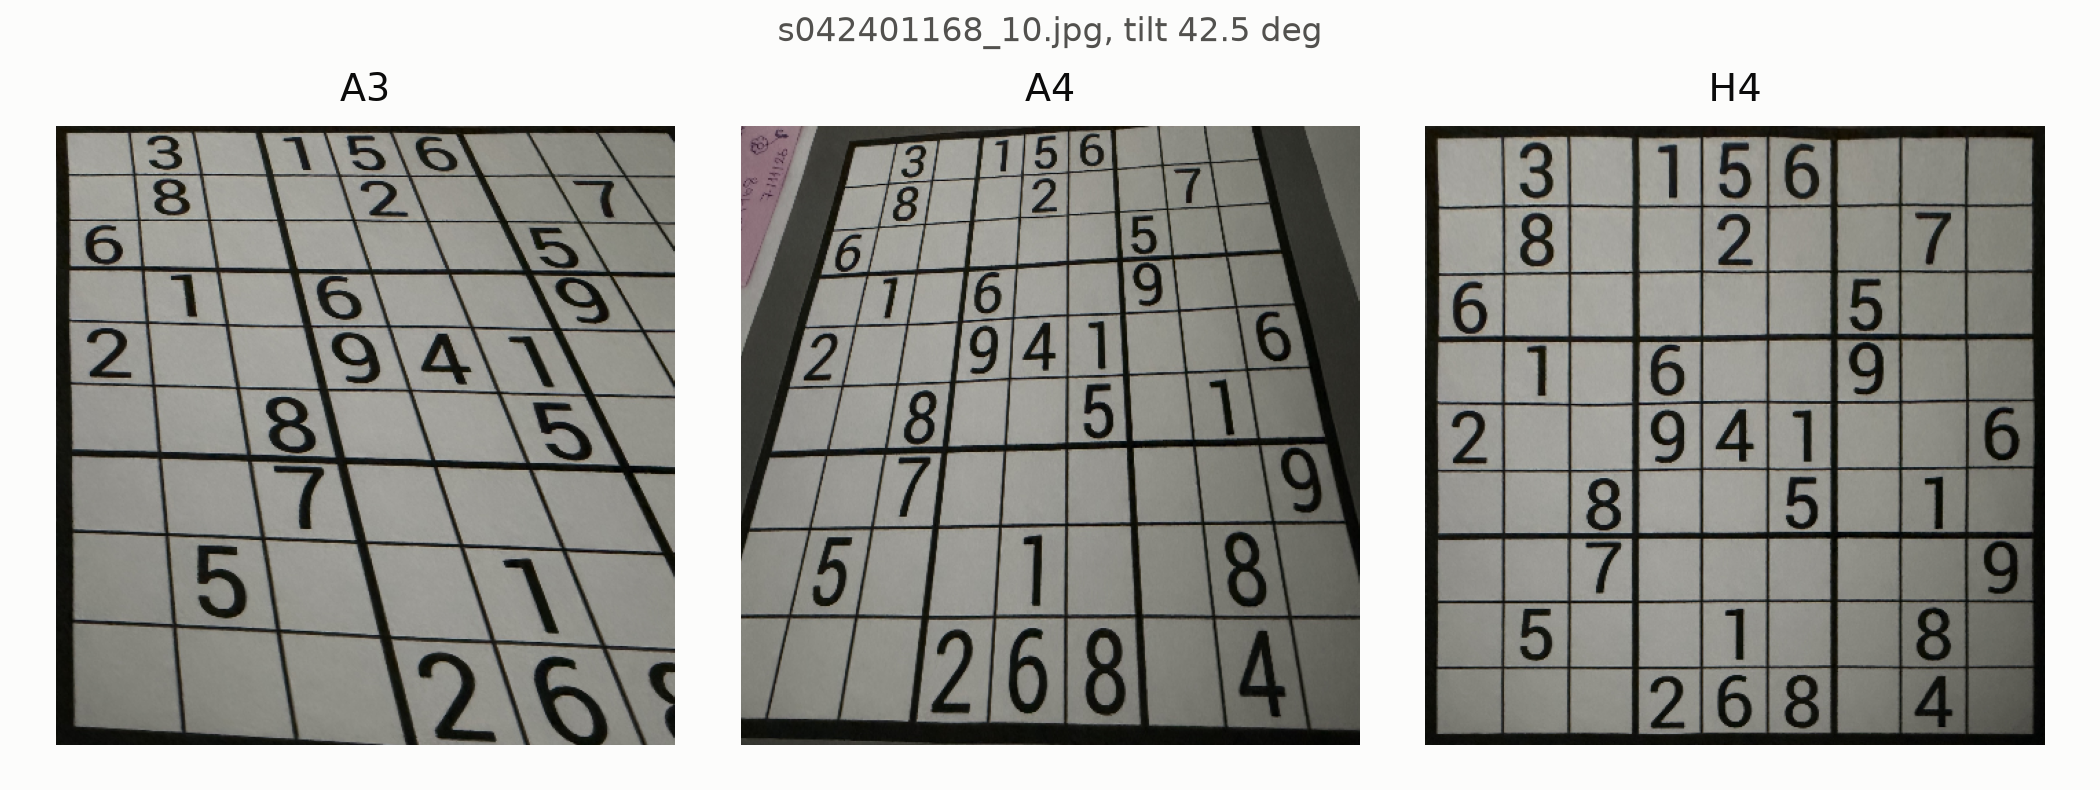
\includegraphics[width=0.72\textwidth]{models_side_by_side.png}
\caption{A3, A4 and H4 rectifications of the most oblique personal photograph (\texttt{s042401168\_10}, tilt $42.5^\circ$). A3 fixes TL, TR and BL exactly and pushes all the error into BR; A4 spreads it over all four corners; only H4 restores parallel, equally spaced grid lines.}
\label{fig:side-by-side}
\end{figure*}



\subsection{Analysis and result}
\begin{table}[t]
\centering\footnotesize
\caption{Stage 4 comparison by tilt (31 images; \texttt{dev\_14} excluded). Each range spans the development-set mean and the personal-set mean.}
\label{tab:tilt}
\scriptsize\setlength{\tabcolsep}{1.6pt}
\begin{tabular}{@{}l r c c c@{}}
\toprule
Tilt & $n$ & Fit error & Spacing error & Cell accuracy\\
 & & A3/A4 (px) & A3/A4/H4 (px) & A3/A4/H4\\
\midrule
$<10^\circ$ & 13 & 12--25/3--6 & 1.8--4.4/1.3--1.6/0.7--1.1 & 0.96--1.00/1.00/1.00\\
$10$--$30^\circ$ & 6 & 68--166/17--34 & 10--19/6--12/0.5--0.7 & 0.72--0.79/0.68--0.94/1.00\\
$\geq30^\circ$ & 12 & 163--236/41--48 & 16--18/13--15/0.9--1.1 & 0.51--0.66/0.56--0.63/$\geq$0.999\\
\bottomrule
\end{tabular}
\end{table}

Near-frontal views give almost identical results for all three models (Table~\ref{tab:tilt}, Fig.~\ref{fig:measures}; per-image values in Table~\ref{tab:compare}, Appendix~\ref{app:tables}). From about $15^\circ$ the affine models break down: lines stay straight but are tilted and unevenly spaced, and OCR accuracy falls to about 60\,\% beyond $30^\circ$. H4 stays at 99.9--100\,\% up to $55^\circ$ (Fig.~\ref{fig:side-by-side}).

A4 cuts the corner residual to about a quarter of A3's, but this does not help OCR. Least squares only spreads the error over the four corners; it cannot undo the uneven cell spacing inside the grid.

The A3 error follows the image-plane distortion more closely than the tilt angle itself (Spearman 0.976 vs.\ 0.929). For example, \texttt{dev\_18} at $42^\circ$ gives 211\,px, while the more oblique \texttt{dev\_20} at $55^\circ$ gives 176\,px.

This is the weak-perspective condition. An affine map is valid while the depth range across the puzzle is small compared with its distance: $\Delta Z/Z_0\approx(L\sin\theta)/Z_0$ for a puzzle of width $L$ tilted by $\theta$. The error therefore grows with both the tilt and how close the camera is. Affine rectification is adequate only for near-frontal views (below about $10^\circ$); beyond that, a homography is required.


% ===========================================================================
\section{Recognition}
\label{sec:recog}
% ===========================================================================
\subsection{Cell extraction and margin}
For recognition, H4 is re-estimated to a $900\times900$ target. At 450\,px a digit is only about 25\,px tall and becomes jagged after upscaling; on the development set the larger warp raised correct reads of filled cells from 552/565 to 560/565. The whole warp is binarised once (division by the blurred background, then a global inverse Otsu threshold); a per-cell Otsu would always split a blank cell into two classes and place its threshold inside the paper texture. Grid lines are then removed with morphological openings by a horizontal and a vertical line of one cell length: grid lines span many cells and survive the opening, digits are shorter than a cell and do not.

The required inner margin is applied in two places. The raw OCR path (used only for the with/without comparison) crops 8\,\% of the cell on each side. The main path looks at a window 15\,\% \emph{larger} than the cell on each side, because with the first, margin-only version the digits of the grey-framed personal puzzle (\texttt{s042401168\_10}--\texttt{12}) reached over the top of their cells and the margin cut them: 3 and 8 were read as 2, 7 was not read, 5 was read as 4, and cell accuracy on the personal set was 99.28\,\% with 7/12 exact grids. After line removal with the larger window those five errors disappeared and the development set did not change.

\subsection{Empty-cell criterion}
The decision is made before OCR from connected components (8-connectivity) of the line-free ink in the window. A component is discarded if its area is below 0.5\,\% of a cell (noise), if it spans the whole window width or height (a remaining line piece), or if its centroid lies outside the central band of its own cell (15--85\,\% in each direction, which excludes a neighbour's digit). The largest remaining component and the parts within 6\,\% of a cell from it are merged, which keeps a broken stroke such as the detached top bar of a 5 in \texttt{dev\_13}. The cell is \emph{filled} if the merged digit is at least 30\,\% of the cell tall and covers at least 2\,\% of its area. Table~\ref{tab:band} (Appendix~\ref{app:tables}) shows that the result is stable: with bands of 0.10 or 0.15 and any window growth between 0 and 0.25 there is no empty-cell error on the development set; wider bands start to lose digits pushed off-centre by the page curl of \texttt{dev\_20}. No setting turned an empty cell into a filled one.



\subsection{OCR configuration and cell preparation}
Tesseract is called through \texttt{pytesseract} with \texttt{-c tessedit\_char\_whitelist=123456789}; 0 is not in the list because empty cells never reach the OCR. Each filled cell is prepared as follows: only the digit component is kept, cropped to its bounding box, scaled to a fixed height, re-thresholded, and centred on a white square canvas with a padding of half the digit height, giving a black digit on white with clean surroundings, the input Tesseract was trained for.

Page-segmentation modes were compared one call per cell (Table~\ref{tab:ocr}). \texttt{--psm 10} (single character) and \texttt{--psm 7} gave identical results, as did \texttt{8} and \texttt{13}; with the LSTM engine of Tesseract~5 the single-character mode appears to be handled like a single line (an observation, not confirmed in the documentation). \texttt{psm 10} returns nothing when unsure, \texttt{psm 8} reads more cells but is wrong more often. Tesseract is also sensitive to digit size: the same ``1'' was read at 24\,px and missed at 40\,px. The final configuration therefore reads every filled cell at three heights (24, 32, 40\,px) with \texttt{psm 10} and \texttt{8} (six reads, run in eight threads) and keeps the most confident reading that passes a set of shape rules (\texttt{digit\_rules.py}): number of holes, vertical position of the hole, and ink on the left side of the upper and middle bands. For example an 8 must have two holes and a 6 may have one hole only in its lower half. These rules removed the last three Tesseract errors on clean, well-prepared digits: \texttt{dev\_18} 5$\to$3, \texttt{s042401168\_06} 9$\to$2 and \texttt{s042401168\_08} 8$\to$3 (Fig.~\ref{fig:ocr-errors}).

\begin{table}[t]
\centering\footnotesize
\caption{OCR configurations. ``Raw'': margin-cropped grey cell without preparation. Unread: filled cells for which OCR returned no digit.}
\label{tab:ocr}
\setlength{\tabcolsep}{4pt}
\begin{tabular}{@{}l l r r r r@{}}
\toprule
Set & Configuration & Cell acc. & Digit acc. & Exact & Unread\\
\midrule
dev & pipeline (6 reads + rules) & 0.9994 & 0.9982 & 19/20 & 0\\
 & psm 10, prepared & 0.9802 & 0.9434 & 10/20 & 30\\
 & psm 8, prepared & 0.9932 & 0.9805 & 13/20 & 7\\
 & psm 10, raw & 0.9235 & 0.7805 & 0/20 & 114\\
\midrule
pers. & pipeline (6 reads + rules) & 1.0000 & 1.0000 & 12/12 & 0\\
 & psm 10, prepared & 0.9722 & 0.9206 & 1/12 & 27\\
 & psm 8, prepared & 0.9928 & 0.9794 & 6/12 & 5\\
 & psm 10, raw & 0.8776 & 0.6500 & 1/12 & 106\\
\bottomrule
\end{tabular}
\end{table}

\begin{figure}[t]
\centering
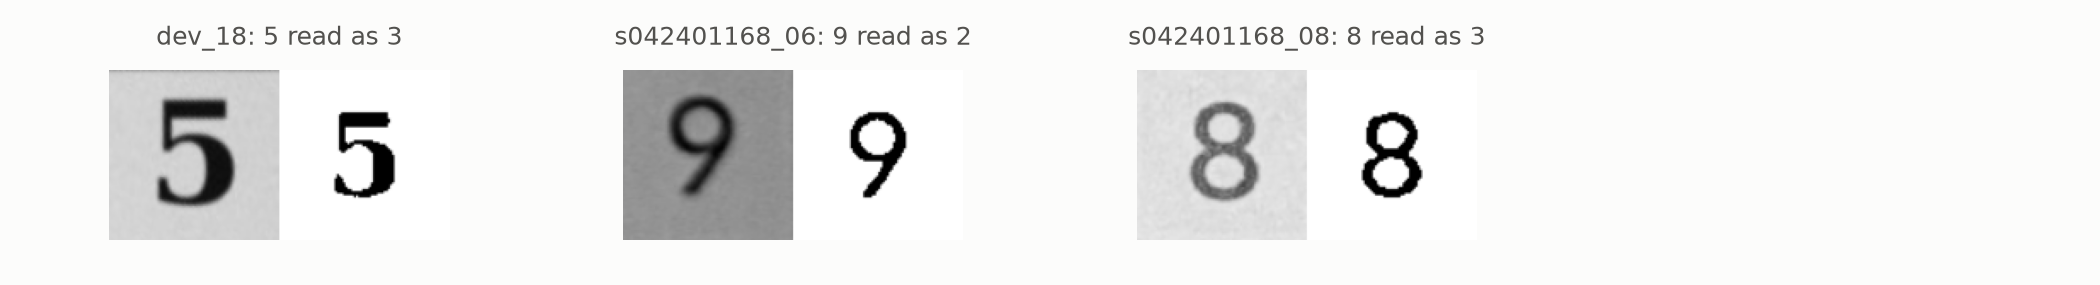
\includegraphics[width=\linewidth]{ocr_errors_before_rules.png}
\caption{The three Tesseract errors left before the shape rules: grey cell (left) and prepared input (right) of each pair.}
\label{fig:ocr-errors}
\end{figure}

\textbf{Effect of preparation.} With the same single \texttt{psm 10} call, preparation raises digit accuracy from 0.78 to 0.94 (dev) and from 0.65 to 0.92 (personal); multiple reads and the shape rules bring cell accuracy to 0.9994 and 1.0000.

\textbf{Confusions.} After the full pipeline only one cell in 2592 is wrong: a 7 in \texttt{dev\_20} (row 7, column 5) is decided \emph{empty}, not misread (Section~\ref{sec:failures}, case~A). The full confusion matrices are in \texttt{out/eval/\{dev,personal\}/confusion.csv}.

\begin{figure*}[t]
\centering
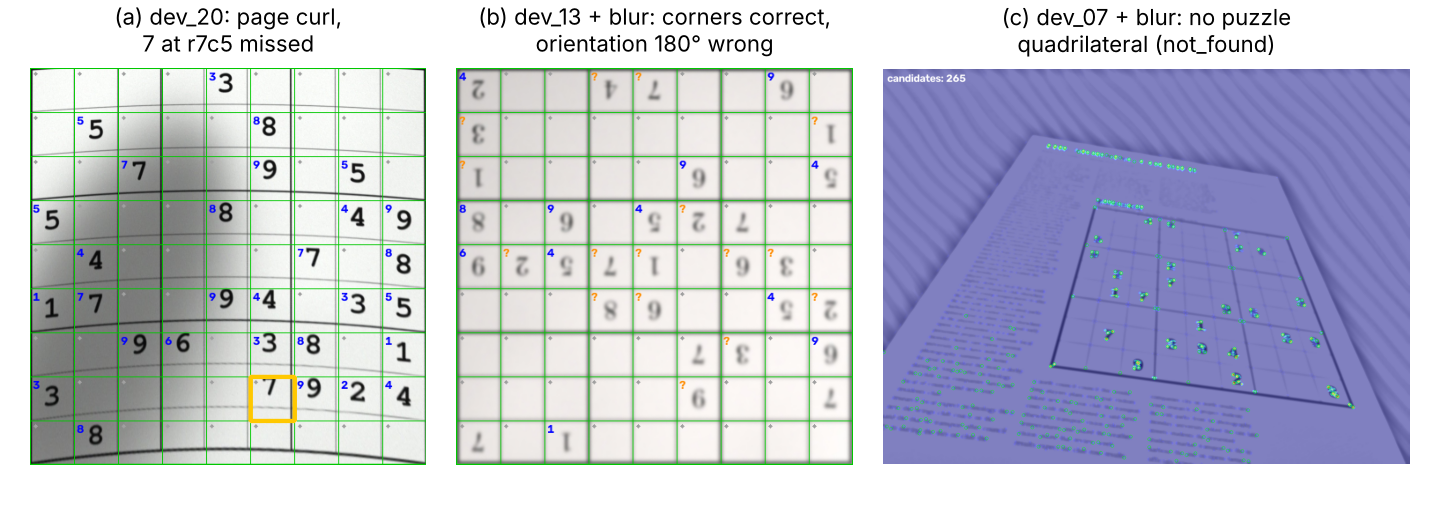
\includegraphics[width=0.75\textwidth]{failures.png}
\caption{Failure cases A--C of Section~\ref{sec:failures} (debug and Harris images).}
\label{fig:failures}
\end{figure*}

\subsection{Validity check}
Every row, column and $3\times3$ box is scanned for repeated non-zero digits; all cells that take part in a repetition are listed, drawn with a red frame in \texttt{\_debug.png}, and the verdict is \texttt{invalid}; otherwise it is \texttt{valid}. All 32 annotated grids are valid sudokus, and all 32 outputs are \texttt{valid}. Before the shape rules, the misreads in \texttt{s042401168\_06} and \texttt{\_08} created repetitions and were flagged \texttt{invalid}, while the 5$\to$3 error in \texttt{dev\_18} did not create one and passed as \texttt{valid}: the check only detects errors that break a rule.

% ===========================================================================
\section{Results}
\label{sec:results}
% ===========================================================================
Table~\ref{tab:metrics} gives the Section~7 metrics on both sets and Table~\ref{tab:cond} (Appendix~\ref{app:tables}) breaks them down by condition C1--C5: every condition reaches a cell accuracy of at least 0.998 on both sets, and the only non-exact grid is \texttt{dev\_20} (C2, C4). The results were reproduced on a second machine (Linux, Tesseract 5.3.4 instead of 5.5.4) with identical grids and corner errors.

\begin{table}[t]
\centering\footnotesize
\caption{Section 7 metrics (means over images; runtime on a laptop).}
\label{tab:metrics}
\setlength{\tabcolsep}{3pt}
\begin{tabular}{@{}l r r r r r r r@{}}
\toprule
Set & Found & Crash & Corner & Cell acc. & F1 & Exact & Time\\
\midrule
dev (20) & 20/20 & 0 & 0.063\,\% & 0.9994 & 0.9995 & 19/20 & 2.13\,s\\
personal (12) & 12/12 & 0 & 0.111\,\% & 1.0000 & 1.0000 & 12/12 & 2.29\,s\\
\bottomrule
\end{tabular}
\end{table}



\textbf{Personal dataset.} Twelve photographs of three printed sources (two books and a grey-framed printout), each with a handwritten card (student number, date) outside the grid. Conditions: C1 three times, C2 four times (up to $42.5^\circ$ tilt), C3, C4 and C5 twice each. The original HEIC files with EXIF are submitted together with the JPEG copies that the pipeline reads. Corners were annotated by hand at $8\times$ zoom with \texttt{analysis/annotate.py}, independently of the pipeline, at the outer corner of the thick border.

\textbf{Robustness.} All 32 annotated images were also run after in-plane rotation, downscaling, blur, strong JPEG compression, darkening and noise (Table~\ref{tab:stress}, Appendix~\ref{app:tables}); ground-truth corners were moved with the same transform. No run crashed. Rotation by $90^\circ$, $180^\circ$ and $270^\circ$ gives the same results as the original, since the orientation step recovers the reading direction. The weak point is blur (Section~\ref{sec:failures}). Seven images without a valid puzzle (blank, noise, an empty box, a crop without the puzzle, an empty sudoku grid, a table and a tic-tac-toe grid) all return \texttt{not\_found}.



\textbf{Runtime.} The mean runtime is 2.1--2.3\,s per image on the development machine, well below the 20\,s limit; on fewer cores it grows (case~E in Section~\ref{sec:failures}).

% ===========================================================================
\section{Failure Analysis}
\label{sec:failures}
% ===========================================================================


\textbf{A. Page curl (\texttt{dev\_20}), Stage 3/5.} The page is curved, so no $3\times3$ transformation can flatten it: after H4 the grid lines are still bent (Fig.~\ref{fig:failures}a; maximum spacing deviation 9\,px against 1--3\,px on flat pages). The bottom rows are pushed towards the lower edge of their cells, and the 7 at row~7, column~5 has its centroid outside the central band, so it is decided empty. This is the only cell error on the 32 images. A fix needs a non-planar model, e.g.\ local homographies from the inner grid intersections (bonus B3).

\textbf{B. Wrong orientation after blur (\texttt{dev\_13}), Stage 5.} The corners are correct, but the $180^\circ$ order is chosen (Fig.~\ref{fig:failures}b; Section~\ref{sec:corners}-E, item~4). Cell accuracy drops to 0.51, yet the verdict is \texttt{valid}: an upside-down grid has no repeated digit, so the validity check cannot detect it.

\textbf{C. No puzzle quadrilateral after blur, Stage 2.} With the same blur, five images (\texttt{dev\_07}, \texttt{dev\_20}, \texttt{s042401168\_03}, \texttt{\_04}, \texttt{\_07}) return \texttt{not\_found} (Fig.~\ref{fig:failures}c); the diagnosis is in Section~\ref{sec:corners}-E, item~4.

\textbf{D. OCR confusion, Stage 5.} \emph{Symptom:} three clean digits were misread: 5 as 3 (\texttt{dev\_18}), 9 as 2 (\texttt{s042401168\_06}) and 8 as 3 (\texttt{s042401168\_08}). The last two created duplicates (\texttt{invalid}). The first did not, so a wrong grid was reported as \texttt{valid}.
\emph{Stage:} rectification, cell extraction and preparation were all correct. The prepared crops are sharp and complete (Fig.~\ref{fig:ocr-errors}). The error is inside Tesseract.
\emph{Diagnosis:} the original chain stopped at the first answer: \texttt{psm 10} at 40\,px digit height. Reading the same crops at 24, 32 and 40\,px with \texttt{psm 10} and \texttt{8} showed that Tesseract also gives the correct digit, with higher confidence (95--96\,\% vs.\ 23--85\,\% for the wrong answer). The wrong answers also contradict simple shape facts: the ``3'' has a full left-upper stroke (1.00; every true 3 is $\leq0.58$), the ``2'' has a hole, and the ``3'' read from an 8 has two holes.
\emph{Fix:} each cell is read six times, and the most confident answer that passes per-digit shape rules (hole count and position, left-side ink) is kept. All three cells are corrected. None of the 905 true digits breaks its rule. Cost: runtime rises from about 1\,s to 2.2\,s per image. The rules were derived from the same data.

\textbf{E. Runtime on a single core, robustness.} The 20\,s limit is met on a laptop (2.2\,s) and on 2 cores (max 12.5\,s) but not on one core (25--27\,s), because each filled cell is read six times and orientation reads 48 cells. Stopping after the first reading that passes the shape rules, or testing only the $0^\circ$ and $180^\circ$ orders when the quadrilateral is roughly upright, would cut the number of calls by a large factor.

% ===========================================================================
\section{Conclusion and Limitations}
% ===========================================================================
On 32 annotated images SudokuScan finds every puzzle (mean corner error 0.081\,\% of the side) and reads 2591 of 2592 cells correctly. The comparison shows that affine models are an acceptable approximation only below about $10^\circ$ of tilt, where depth variation across the puzzle is negligible, and that the homography is necessary for oblique photos.

\textbf{Limitations.} Thresholds were tuned on the reported 32 images (the 12 personal photos are only a small independent check); curved pages are outside the planar model; strong blur breaks corner selection and orientation; the OCR relies on hand-made shape rules; runtime depends on the number of CPU cores.

% ===========================================================================
\appendices
\section{AI-Use Disclosure (Appendix C of the brief)}
% ===========================================================================
{\footnotesize
\setlength{\tabcolsep}{3pt}
\begin{tabularx}{\linewidth}{@{}>{\raggedright\arraybackslash}p{1.1cm} >{\raggedright\arraybackslash}p{1.25cm} >{\raggedright\arraybackslash}X >{\raggedright\arraybackslash}p{2.3cm}@{}}
\toprule
Tool & Purpose / stage & What I asked (summary) & Kept, changed or rejected\\
\midrule
Claude (claude.ai) & Planning (all) & Split the project into phases with a checklist and schedule; suggested a folder structure & Kept the phase plan and checklist\\
Claude (claude.ai) & Learning (all stages) & Explained the concepts of each phase; clarified what I did not understand in my own reading; edited my research notes (\texttt{phases/*.md}) & Kept the explanations; the notes are my research, edited for clarity\\
Claude (claude.ai) & Code (all stages) & Example skeleton with a TODO list for each module; reviewed my code phase by phase & Wrote the code myself from the TODOs; errors found in review were fixed together\\
Claude (claude.ai) & Stage 2, Stage 4 & I described my algorithm; where I got stuck, Claude suggested how to write it in code. Claude prepared and ran the test and evaluation scripts and reported the results & The selection rule and the conclusions are mine; tests and measurements were prepared and run with Claude\\
Claude Code & Setup & Example skeleton at the first setup & Rejected; deleted in Phase 1\\
Claude Code & Testing & End-to-end runs of the whole program under conditions I specified, several times & Used the results to find failures\\
Claude Code & README & Rewrote \texttt{README.md}; added the Tesseract note to \texttt{requirements.txt} & Kept after checking\\
Claude (claude.ai) & Report & Writing assistant (English, IEEE format): drafted Sections I, III, V--VIII from my notes and results, laid out tables and figures, checked the numbers, re-ran the pipeline on a second machine; language and formatting of my Stage 2 and 4 text & Kept the drafts after review; Stage 2 and Stage 4 text written by me\\
\bottomrule
\end{tabularx}
}

\vspace{1ex}
\noindent\footnotesize\textbf{Working rule for Stages 2 and 4.} From Phase~2 on, every Claude Code session started with the rule shown in Fig.~\ref{fig:cc-rules}: the selection logic (puzzle region, choice of the four corners, ordering, \texttt{not\_found} criterion) is written by me; Claude Code only follows, helps with auxiliary tools (test and evaluation scripts) and reviews. I also asked it to stop me if I ever asked it to write those parts. The same rule is recorded in the project notes (\texttt{calisma-duzeni.md}).

\begin{figure}[h]
\centering
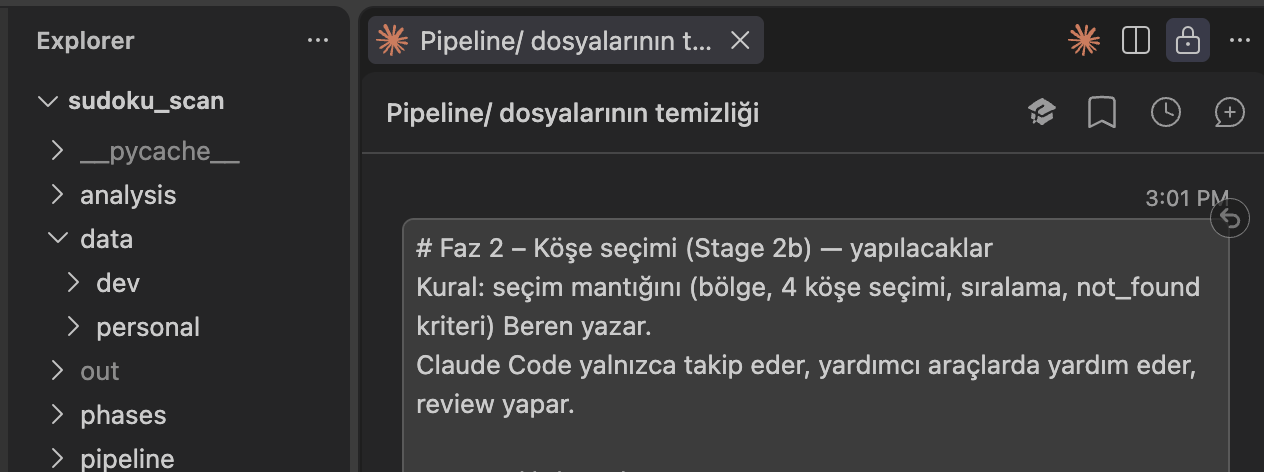
\includegraphics[width=0.9\linewidth]{claude_code_rules.png}
\caption{Start of the Phase 2 Claude Code session (in Turkish): ``Rule: Beren writes the selection logic (region, choice of the four corners, ordering, \texttt{not\_found} criterion). Claude Code only follows, helps with auxiliary tools and reviews.''}
\label{fig:cc-rules}
\end{figure}

\vspace{1ex}
\noindent\footnotesize I confirm that I wrote the corner-selection logic and the comparison analysis myself, and that I can explain and modify every part of my submission.

\vspace{2ex}
\noindent Name: Zeyneb Beren Kece \hfill Student no.: 042401168\\[2ex]
Signature: \rule{3.5cm}{0.4pt} \hfill Date: \rule{2.2cm}{0.4pt}


\section{Additional Tables}
\label{app:tables}
\begin{table}[h]
\centering\footnotesize
\caption{Harris parameter study, one parameter at a time (8 images). Errors are mean corner error in \% of the puzzle side; ``peak'' is before and ``final'' after \texttt{cornerSubPix}. None of the settings produced a \texttt{not\_found}.}
\label{tab:harris}
\begin{tabular}{@{}l l r r r r@{}}
\toprule
Parameter & Value & Cand. & Peak & Final & Worst\\
\midrule
blockSize (ratio) & 0.003 & 454 & 0.401 & 0.059 & 0.125\\
 & \textbf{0.004} & 378 & 0.508 & 0.059 & 0.124\\
 & 0.005 & 317 & 0.775 & 0.274 & 0.883\\
 & 0.007 & 242 & 0.984 & 0.856 & 1.003\\
 & 0.012 & 170 & 1.745 & 1.693 & 2.475\\
\midrule
ksize & \textbf{3} & 378 & 0.508 & 0.059 & 0.124\\
 & 5 & 348 & 0.513 & 0.059 & 0.124\\
 & 7 & 322 & 0.507 & 0.059 & 0.124\\
\midrule
$k$ & 0.02 & 387 & 0.505 & 0.059 & 0.124\\
 & \textbf{0.04} & 378 & 0.508 & 0.059 & 0.124\\
 & 0.06 & 374 & 0.504 & 0.059 & 0.124\\
 & 0.08 & 372 & 0.507 & 0.059 & 0.124\\
 & 0.12 & 364 & 0.546 & 0.076 & 0.240\\
\midrule
Threshold & 0.001 & 879 & 0.508 & 0.059 & 0.124\\
($\times R_{\max}$) & 0.005 & 559 & 0.508 & 0.059 & 0.124\\
 & \textbf{0.01} & 378 & 0.508 & 0.059 & 0.124\\
 & 0.05 & 208 & 0.508 & 0.059 & 0.124\\
 & 0.1 & 166 & 0.508 & 0.059 & 0.124\\
\midrule
cornerSubPix & off & 378 & 0.508 & 0.508 & 0.759\\
window (px) & 2 & 378 & 0.508 & 0.175 & 0.282\\
 & \textbf{3} & 378 & 0.508 & 0.059 & 0.124\\
 & 5 & 378 & 0.508 & 0.177 & 0.357\\
 & 8 & 378 & 0.508 & 0.335 & 0.522\\
\bottomrule
\end{tabular}
\end{table}
\begin{table}[h]
\centering\footnotesize
\caption{Perturbed copies of the 32 annotated images.}
\label{tab:stress}
\setlength{\tabcolsep}{4pt}
\begin{tabular}{@{}l r r r r@{}}
\toprule
Perturbation & Found & Corner mean / max (\%) & Cell acc. & Exact\\
\midrule
original & 32/32 & 0.081 / 0.183 & 0.9996 & 31/32\\
rotation 90/180/270 & 32/32 & 0.081 / 0.184 & 0.9996 & 31/32\\
rotation $45^\circ$ & 32/32 & 0.150 / 0.739 & 1.0000 & 32/32\\
scale 50\,\% & 32/32 & 0.104 / 0.220 & 0.9992 & 30/32\\
scale 25\,\% & 31/32 & 0.217 / 0.469 & 0.9968 & 28/32\\
blur ($\sigma=2$\,px) & 27/32 & 5.361 / 141.3 & 0.9634 & 14/32\\
JPEG quality 20 & 32/32 & 0.085 / 0.188 & 0.9985 & 28/32\\
dark ($\gamma=2.5$) & 31/32 & 0.142 / 1.142 & 0.9996 & 30/32\\
noise ($\sigma=15$) & 31/32 & 0.090 / 0.261 & 0.9980 & 27/32\\
\bottomrule
\end{tabular}
\end{table}
\begin{table}[h]
\centering\footnotesize
\caption{Empty-cell decision on the development set (1620 cells) for different centre bands; the result was identical for every window growth from 0 to 0.25.}
\label{tab:band}
\begin{tabular}{@{}r r r r@{}}
\toprule
Band & F1 (empty) & Empty$\to$filled & Filled$\to$empty\\
\midrule
0.10 & 1.0000 & 0 & 0\\
\textbf{0.15} & 1.0000 & 0 & 0\\
0.20 & 0.9995 & 0 & 1\\
0.25 & 0.9976 & 0 & 5\\
\bottomrule
\end{tabular}
\end{table}
\begin{figure}[h]
\centering
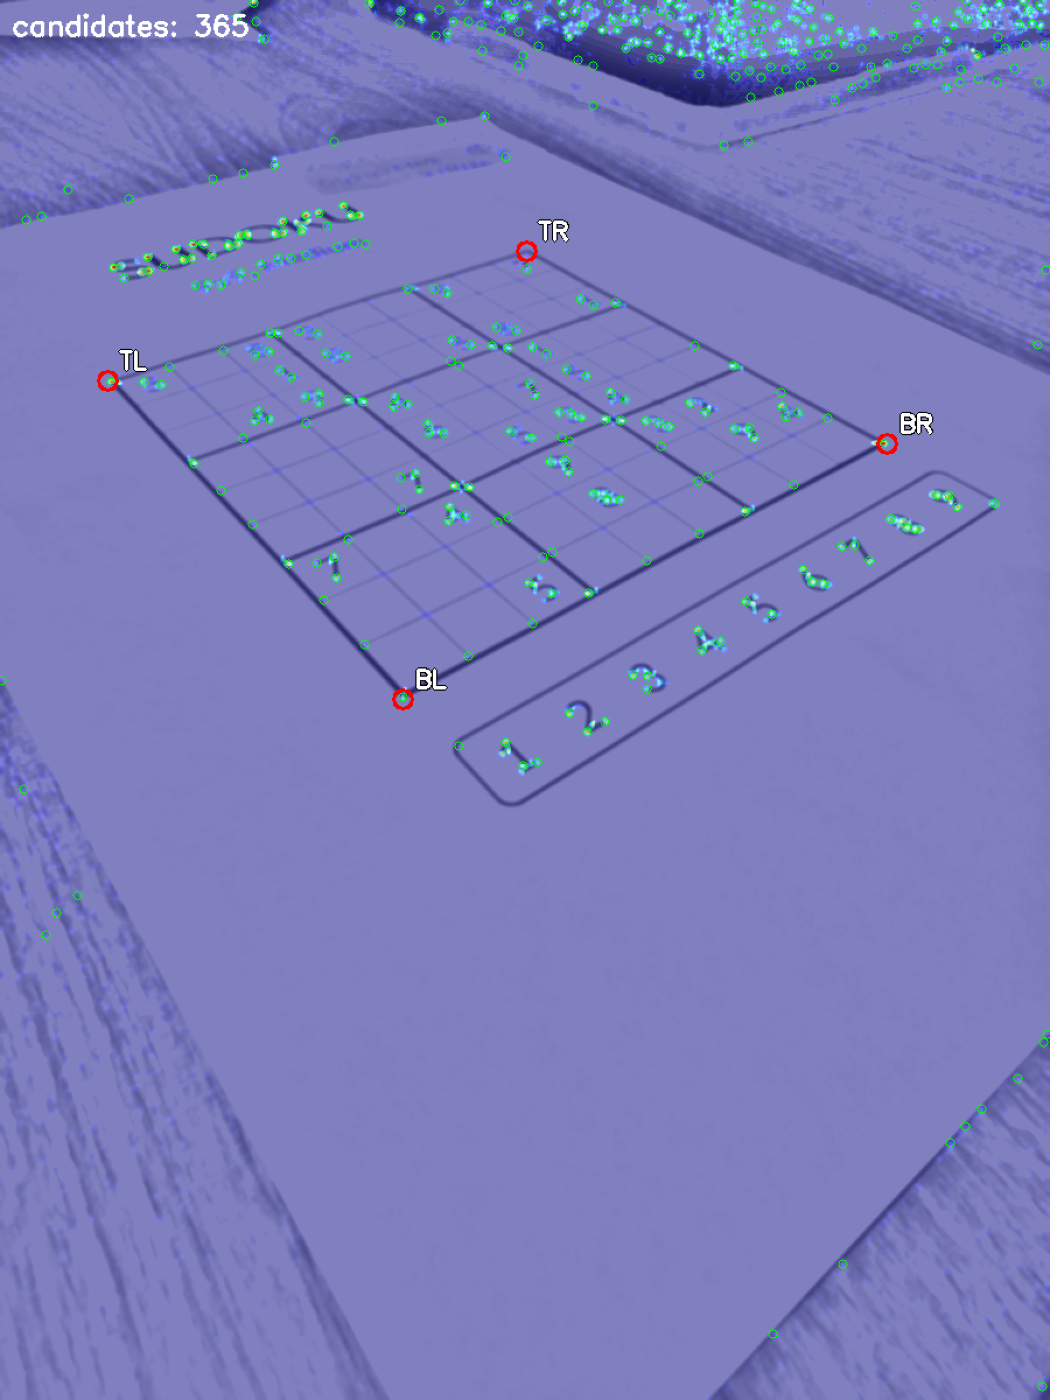
\includegraphics[width=0.5\linewidth]{harris_example.png}
\caption{Harris response (colour), all 365 candidates (green) and the four selected corners (red) on an oblique development image. The candidates include digits, the title, the number strip and the background; the selection rule has to ignore them.}
\label{fig:harris}
\end{figure}
\begin{table}[h]
\centering\footnotesize
\caption{Selected images from \texttt{out/eval/compare\_*.csv}: fit error (A3 fourth-corner error, A4 RMS, H4 max), mean grid-spacing deviation and OCR cell accuracy.}
\label{tab:compare}
\setlength{\tabcolsep}{3pt}
\begin{tabular}{@{}l r r r r r r r r r@{}}
\toprule
 & & \multicolumn{3}{c}{Fit err.\ (px)} & \multicolumn{2}{c}{Spacing (px)} & \multicolumn{3}{c}{Cell acc.}\\
\cmidrule(lr){3-5}\cmidrule(lr){6-7}\cmidrule(l){8-10}
Image & Tilt & A3 & A4 & H4 & A4 & H4 & A3 & A4 & H4\\
\midrule
s\_05 & 0.6 & 2.4 & 0.6 & 0 & 0.56 & 0.56 & 1.00 & 1.00 & 1.00\\
dev\_01 & 3.6 & 15.7 & 4.0 & 0 & 0.67 & 0.56 & 0.99 & 1.00 & 1.00\\
dev\_19 & 9.5 & 38.6 & 10.3 & 0 & 4.06 & 0.61 & 0.94 & 1.00 & 1.00\\
dev\_13 & 16.9 & 72.5 & 16.3 & 0 & 4.17 & 0.78 & 0.85 & 0.96 & 1.00\\
dev\_16 & 21.5 & 83.6 & 19.8 & 0 & 5.67 & 0.56 & 0.67 & 0.82 & 1.00\\
s\_02 & 24.3 & 165.8 & 34.1 & 0 & 12.06 & 0.50 & 0.72 & 0.68 & 1.00\\
dev\_05 & 36.3 & 110.4 & 30.6 & 0 & 8.56 & 0.78 & 0.74 & 0.78 & 1.00\\
s\_10 & 42.5 & 390.7 & 63.0 & 0 & 13.44 & 1.83 & 0.53 & 0.49 & 1.00\\
dev\_07 & 52.3 & 256.9 & 49.7 & 0 & 18.94 & 0.56 & 0.62 & 0.54 & 1.00\\
dev\_20 & 55.5 & 175.6 & 54.2 & 0 & 10.67 & 1.50 & 0.57 & 0.56 & 0.99\\
\bottomrule
\end{tabular}
\end{table}
\begin{table}[h]
\centering\footnotesize
\caption{Results by condition. An image with several conditions is counted in each of its rows.}
\label{tab:cond}
\setlength{\tabcolsep}{4pt}
\begin{tabular}{@{}l l r r r r r@{}}
\toprule
Set & Cond. & $n$ & Corner (\%) & Cell acc. & F1 & Exact\\
\midrule
dev & C1 near-frontal & 5 & 0.050 & 1.0000 & 1.0000 & 5/5\\
 & C2 oblique & 9 & 0.094 & 0.9986 & 0.9989 & 8/9\\
 & C3 rotation & 4 & 0.045 & 1.0000 & 1.0000 & 4/4\\
 & C4 lighting & 6 & 0.050 & 0.9979 & 0.9984 & 5/6\\
 & C5 clutter & 6 & 0.049 & 1.0000 & 1.0000 & 6/6\\
\midrule
pers. & C1 near-frontal & 3 & 0.096 & 1.0000 & 1.0000 & 3/3\\
 & C2 oblique & 4 & 0.131 & 1.0000 & 1.0000 & 4/4\\
 & C3 rotation & 2 & 0.109 & 1.0000 & 1.0000 & 2/2\\
 & C4 lighting & 2 & 0.106 & 1.0000 & 1.0000 & 2/2\\
 & C5 clutter & 2 & 0.124 & 1.0000 & 1.0000 & 2/2\\
\bottomrule
\end{tabular}
\end{table}
\begin{figure}[h]
\centering
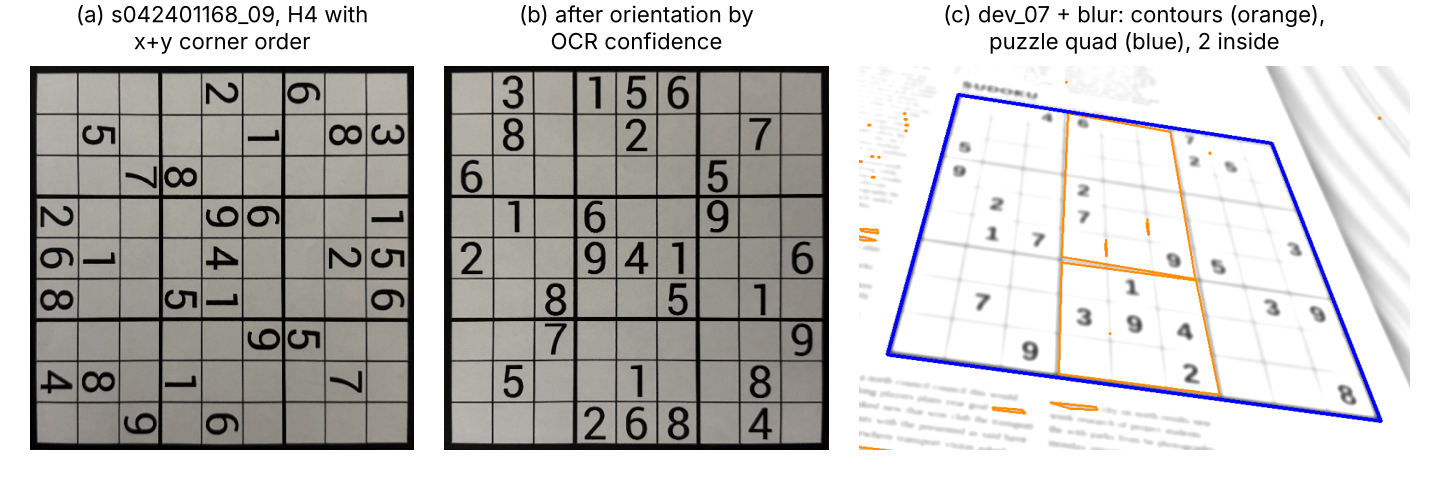
\includegraphics[width=\linewidth]{corner_failures.png}
\caption{Corner-stage failures. (a) H4 of \texttt{s042401168\_09} with the corner order from $x+y$: the grid is sideways. (b) The same image after choosing the order by OCR confidence. (c) Blurred \texttt{dev\_07}: closed contours (orange) and the puzzle quadrilateral (blue), which contains only 2 smaller quadrilaterals.}
\label{fig:corner-failures}
\end{figure}
\end{document}
